\section{Physics Beyond the Standard Model}

The SM predicts numerous phenomena (e.g.\ the existence of the $Z$ and Higgs
boson) that could only be experimentally verified decades after its
formulation. However, the SM is known to be incomplete for several reasons:
\begin{description}

\item[Matter-antimatter asymmetry] In the Big Bang cosmological model, equal
  amounts of matter and antimatter are produced in the initial phase of the
  evolution of the universe. However, the universe observed today mostly
  consists of matter particles, thus resulting in a large asymmetry between
  matter and antimatter. The SM does not contain a mechanism that can explain
  the size of the matter-antimatter asymmetry observed in the universe.

\item[Gravitation] At the moment, no quantum field theory of gravitation exists
  that could be incorporated into the SM. Therefore, the SM does not attempt to
  describe gravitational interactions between massive particles. In addition, it
  is currently not understood why the gravitational interaction between
  elementary particles is much weaker than the strong or electroweak
  interaction.

\item[Dark matter] Based on astrophysical observations it is postulated that the
  vast majority of the universe consists of a form of matter, referred to as
  dark matter, that interacts gravitationally but not electromagnetically.

  The SM does not provide a dark matter candidate particle.

\item[]

\item[Neutrinos] Mass, Majorana, Dirac, etc.

\end{description}



\begin{description}

\item[Vacuum Stability] The present minimum with a vacuum expectation
  value of $v \approx \si{246}{\GeV}$ might be either a global minimum
  in which case the universe is stable or only a local minimum which
  leads to a metastable universe. In the metastable case, the state of
  the Higgs field could tunnel to a new local or global minimum with a
  smaller vacuum expectation value. Current experimental data cannot
  distinguish whether the universe is stable or
  meta-stable\todo{citation}.

\item[Elektroweak phase transition] In baryogenesis a first order
  electroweak phase transition is needed.

\end{description}


\subsection{Non-Resonant Higgs Boson Pair Production}

\begin{figure}[htbp]
  \centering

  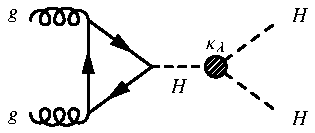
\includegraphics[width=0.35\textwidth]{feynman_graphs/di_higgs_effective}

  \caption{Non-resonant production of Higgs boson pairs in BSM}%
  \label{fig:bsm_hh_prod_feyn}
\end{figure}



New physics at high energy scales

So high that new particles cannot be produced directly.

However, new particles can appear virtually in higher order corrections such as
loops etc.

If the mass scale of these particles is sufficiently large, can express the new
physics as an effective theory extending the SM.

\Cref{fig:bsm_hh_prod_feyn}



\subsection{Resonant Higgs Boson Pair Production}


\begin{figure}[htbp]
  \centering

  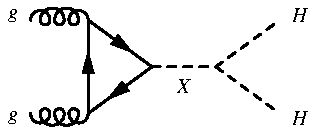
\includegraphics[width=0.35\textwidth]{feynman_graphs/di_higgs_resonant}

  \caption{Resonant production of Higgs boson pairs}%
  \label{fig:resonant_production_feyn}
\end{figure}



\todo[inline]{What models predict Spin-0 resonances decaying into pair of SM
  Higgs? 2HDM}

\todo[inline]{Mention Spin-2 resonances? KK-graviton -- theoretically not favoured}

% \item[BSM] Radions, 2HDM, Warped extra dimensions, composite Higgs, hMSSM, KK
%   Gravitons: Most could decay to pairs of SM Higgs bosons.

\todo[inline]{1 page}


%%% Local Variables:
%%% mode: latex
%%% TeX-master: "../../phd_thesis"
%%% End:
